\documentclass[11pt,a4paper,twoside]{article}

% ---------------- IMPORTE -----------------------------
\usepackage[german]{babel}
\usepackage{blindtext}
\usepackage{color}
\usepackage{graphicx}
\usepackage{fancyhdr}
\usepackage[left=25mm, right=25mm, top=25mm, bottom=33mm]{geometry} % Seitenränder
\usepackage{parskip}
\usepackage{tabularx,colortbl}
\usepackage{wrapfig}
\usepackage{epstopdf}
\usepackage{minted}
%\usepackage[font={small,it}]{caption}
%\usepackage{colortbl}
%\usepackage{listings}
\usepackage[utf8]{inputenc}
\usepackage{tocloft}
\usepackage{setspace}
\usepackage{tcolorbox}
\usepackage{subfig}
\usepackage{prettyref}
\usepackage{enumitem}
\usepackage{bold-extra}
\usepackage{hyperref}

% --------------- Klickbare Links --------------------------
\hypersetup{
    colorlinks=true,
    linktoc=all,
    linkcolor=black,
}

% --------------- Querverweis --------------------------
\newrefformat{fig}{Abbildung \ref{#1}}
\newrefformat{sec}{\ref{#1}}

% --------------- Common-Settings ----------------------
\epstopdfsetup{outdir=./}
\setlength{\abovecaptionskip}{5px}
\setlength{\belowcaptionskip}{0pt}
\setlength{\extrarowheight}{4pt}
\setlength{\cftfigindent}{0px}
\captionsetup{justification=centering}

% --------------- CODE-Beispiele -----------------------
\definecolor{bg}{rgb}{0.85,0.85,0.85}
\tcbuselibrary{minted,skins}
\newtcblisting{javacode}[1][]{
  listing engine=minted,
  colback=bg,
  colframe=black!70,
  listing only,
  minted style=friendly,
  minted language=java,
  minted options={linenos=true,fontsize=\footnotesize,numbersep=2mm,texcl=true,#1},
  left=5mm,enhanced,
  top=0mm, bottom=0mm,
  overlay={\begin{tcbclipinterior}\fill[black!25] (frame.south west)
            rectangle ([xshift=5mm]frame.north west);\end{tcbclipinterior}}
}

% --------------- ADITO-spezifische Farben -------------
\definecolor{ADITO_RED}{rgb}{0.93,0.09,0.32}

% --------------- Neuer Spaltentyp ---------------------
\newcolumntype{P}[1]{>{\centering\arraybackslash}p{#1}} %zentriert eine Spalte mit fester Breite

% ---------------- Seitenzahlen rechts + Logo ----------
\pagestyle{fancy}
\fancyhf{}

\fancyhead[L]{\textbf{\textsc{Shortcut-Editor}} \\ Implementierung eines Editors zur Bearbeitung von Tastaturkürzeln}
\fancyhead[R]{\vspace{-5mm}
\includegraphics[height=0.045\textheight]{../img/ADITO_Logo}}
\fancyfoot[LE,RO]{\thepage}
\fancyfoot[LO,RE]{\copyright\ Korbinian Mifka}

\renewcommand{\headrulewidth}{1pt}
\renewcommand{\footrulewidth}{1pt}
% ------------------------------------------------------
% ------------------------------------------------------
\begin{document}
\begin{titlepage}

\begin{center}

\includegraphics[scale=0.25]{../img/LogoIHK.pdf}\\[1ex]
\Large{Abschlussprüfung Sommer 2018}\\[3ex]

\Large{Fachinformatiker für Anwendungsentwicklung}\\
\LARGE{Dokumentation zur betrieblichen Projektarbeit}\\[4ex]

\huge{\textbf{Shortcut-Editor}}\\[1.5ex]
\Large{\textbf{Implementierung eines Editors zur Bearbeitung von Tastaturkürzeln}}\\[4ex]

\normalsize
\begin{tabularx}{0.54\textwidth}{rl}
Abgabetermin: & 18.05.2018 \\
Projektverantwortlicher: & Robert Loipfinger\\
\end{tabularx}
\\[3em]

\textbf{Prüfungsbewerber:}\\
Korbinian Mifka\\

\vfill


\includegraphics[scale=0.7]{../img/ADITO_Logo}\\[2ex]
\textbf{Ausbildungsbetrieb:}\\
ADITO Software GmbH\\
Konrad Zuse Str. 4\\
84144 Geisenhausen\\[5em]
\end{center}

\small
\noindent
Dieses Werk einschließlich seiner Teile ist \textbf{urheberrechtlich geschützt}.
Jede Verwertung außerhalb der engen Grenzen des Urheberrechtgesetzes ist ohne
Zustimmung des Autors unzulässig und strafbar. Das gilt insbesondere für
Vervielfältigungen, Übersetzungen, Mikroverfilmungen sowie die Einspeicherung
und Verarbeitung in elektronischen Systemen.

\end{titlepage}
\pagenumbering{gobble}
\tableofcontents
\thispagestyle{fancy}
\newpage

\pagenumbering{arabic}
\setcounter{page}{1}
\section{Vorwort}
\subsection{ADITO Software GmbH}
\begin{wrapfigure}[8]{r}[0cm]{180px}
	\vspace{-8px}
	\centering
	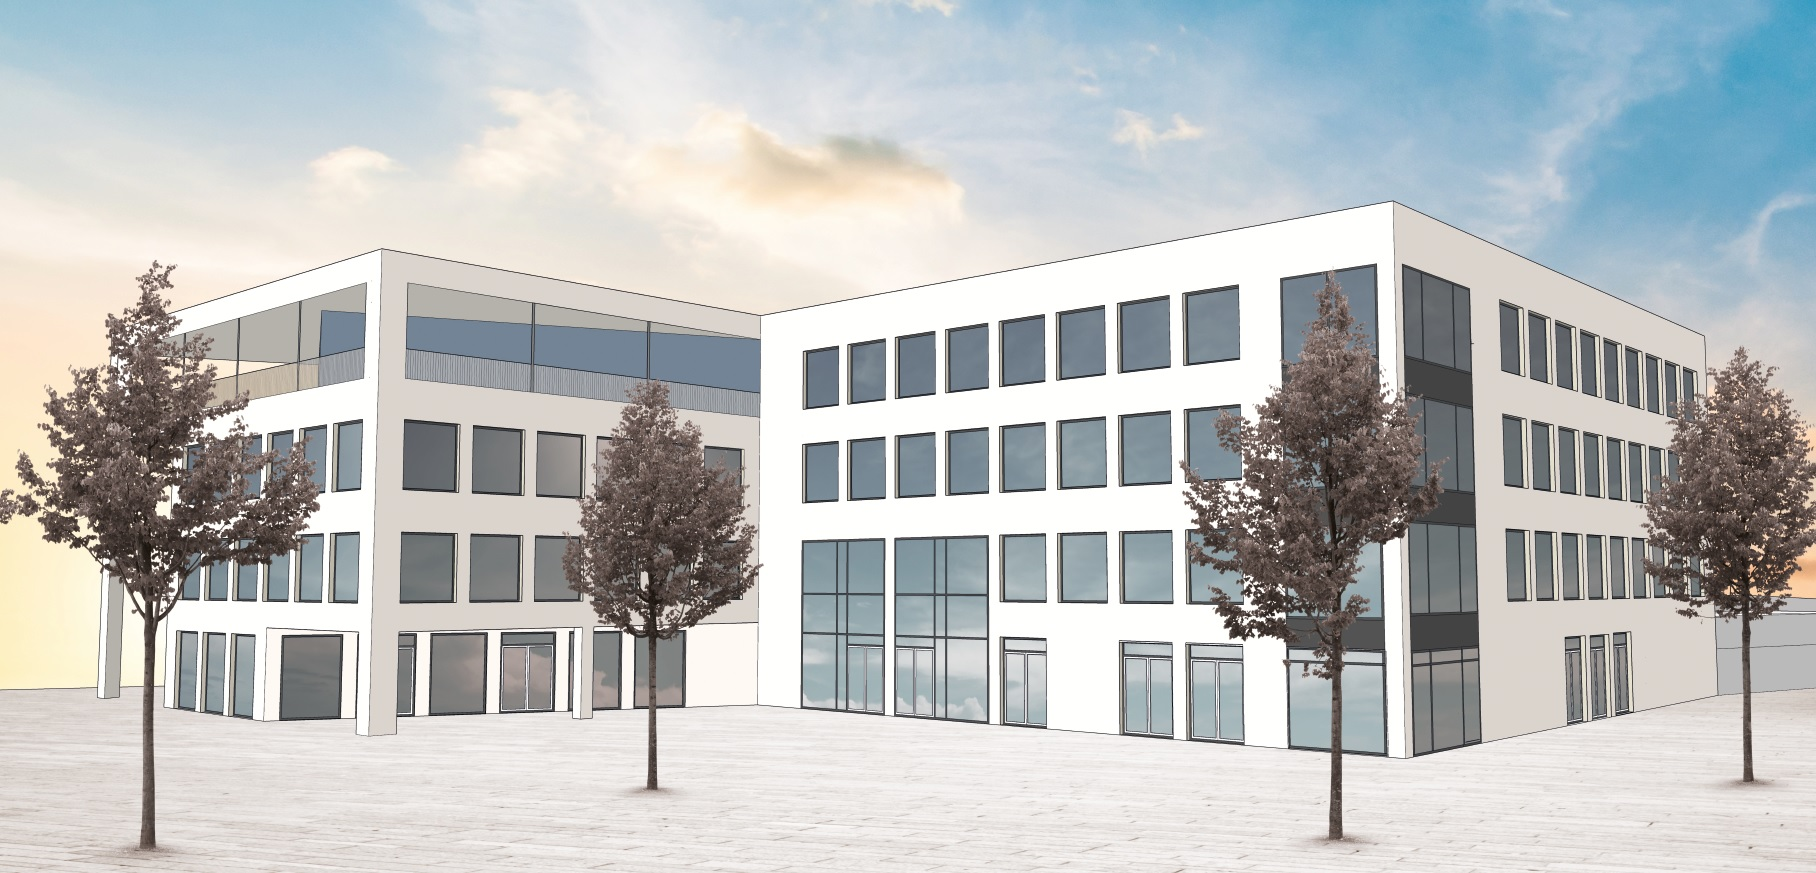
\includegraphics[width=175px]{../img/Firmengebaeude}
	\caption{Firmengebäude}
\end{wrapfigure}

Die ADITO Software GmbH zählt zu den führenden Herstellern hochflexibler Business-, CRM- und xRM-Software. ADITO bietet Entwicklung, Vertrieb, Projektierung und Service aus einer Hand. Das inhabergeführte Unternehmen legt großen Wert auf die persönliche Beratung und Kundenbetreuung durch ihre exzellent ausgebildeten Mitarbeiter.

Kunden von ADITO kommen aus den unterschiedlichsten Branchen. Neben namhaften mittelständischen Unternehmen, zum Beispiel Ravensburger, Birco oder Erlus, gehören auch große Organisationen wie die WWK Versicherungsgruppe, IG Metall, Kassenärztliche Vereinigungen oder die Bundesagentur für Arbeit zu unseren Referenzen. Insgesamt setzen rund 800 Kunden auf Service, Innovationsstärke und Kontinuität von ADITO.

\subsection{Intention}
\par 
In der neuesten Version des xRM-Systems ADITO5 wurde eine neue Clientvariante entwickelt. Nun ist es möglich neben dem konventionellen Java Swing Client einen Webclient bzw. Browserclient einzusetzen. Dieser bietet einige Vorteile. Beispielsweise ist keine Installation mehr notwendig und er kann auf allen Geräten (PC, Tablet und Smartphone) genutzt werden. Allerdings gehen damit auch einige Herrausforderungen einher. So auch bei der Vergabe von Tastaturkürzeln. Browser behalten es sich vor, einige Shortcuts für eigene Aktionen zu reservieren und so nicht für die eigendliche Webanwendung zur Verfügung zu stellen. Beispiele für solche Shortcuts währen Strg + P für Drucken oder Strg + F für Suchen. Der Überblick über die Verwendbarkeit von Tastaturkürzeln geht schnell verloren, da diese in jeder Browser Betriebssystem permutation variieren kann.

Um den Projektierern unserer xRM-Software die Vergabe von Shortcuts zu erleichtern soll ein spezieller Shortcut-Editor entwickelt werden, der die Eingabe und Bearbeitung von Shortcuts per Tastatur und Maus ermöglicht und bei der Wahl des passenden Shortcuts Unterstützung bietet.
Dafür soll bei Tastaturkürzeln gewahrnt werden, wenn sie auf einem Browser Probleme breiten könnten.
Um feststellen zu können warum ein Shortcut problematisch ist, sollen weitere Informationen angezeigt werden, welche beispielsweise angeben, in welchem Browser bzw. welcher Version das Tastaturkürzel bereits verwendet wird.
\par
\newpage
\section{Analysephase}

\begin{wrapfigure}[11]{r}[0cm]{170px}
	\vspace{-12px}
	\centering
	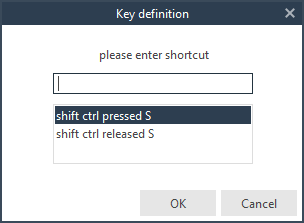
\includegraphics[width=170px]{../graphic/images/screenshots/Alter-Editor}
	\caption{Bestehender Editor}
	\label{fig:existEditor}
\end{wrapfigure}

\subsection{Ist-Analyse}

Seit früheren Versionen existierte bereits ein Editor zur Eingabe von Shortcuts (siehe \autoref{fig:existEditor}). Dieser ist allerdings sehr einfach aufgebaut und beschränkt sich auf die Eingabe eines Shortcuts per Tastatur. Außerdem ist es nicht möglich Warnungen anzuzeigen oder zwischen bestehenden Shortcuts zu navigieren. Da dieser Editor in keinerlei Hinsicht den gegebenen Anforderungen dieses Projekts entspricht, wurde eine Weiterentwicklung dessen vom Autor als nicht sinnvoll erachtet.

Die Aktionen, welchen Shortcuts zugeordnet werden sollen, sind im ADITO Designer schon vorhanden. Zudem existieren sogenannte Entitys, welche Dateneinheiten darstellen und eben genannte Aktionen besitzen können. Beispielsweiße könnte ein Entity \glqq Person\grqq\xspace existieren, welches wiederum die Aktion \glqq Person hinzufügen\grqq\xspace besitzt. Dieser Aktion könnte nun ein Shortcut zugewiesen werden z.B. Strg + Einfg.

\subsection{Sollkonzept}

Der neue Editor muss ebenfalls die Eingabe aber auch die Bearbeitung (z.B. Entfernen einer einzelnen Taste) eines Shortcuts per Tastatur und Maus unterstützen. Für die Navigation und für einen besseren Überblick, werden alle bestehenden Tastenkombinationen in tabellarischer Form präsentiert. Es soll zu jedem Zeitpunkt ersichtlich sein, für welche Aktion der Shortcut definiert wird. Eine weitere Anforderung besteht darin, alle Warnungen für die entsprechenden Browser und deren Betriebssysteme anzuzeigen.

\subsection{Anwendungsfälle}

Um eine grobe Übersicht über alle Anwendungsfälle zu erhalten, die von dem umzusetzenden Editor
abgedeckt werden sollen, wurde im Laufe der Analysephase ein Use-Case-Diagramm erstellt. Dieses
Diagramm befindet sich im Anhang \ref{usecase}.

\subsection{\glqq Make or Buy\grqq -Entscheidung}
Am Ende der Analysephase wurde sich die Frage gestellt, ob der Editor selber entwickelt oder gekauft werden soll. Dazu wurde der Markt nach Software durchsucht, welche den Anforderungen dieses Projekts entspricht. Da diese Suche zu keinem Ergebnis gekommen war, wurde sich für die eigene Entwicklung des Editors entschieden.

\newpage

\section{Projektablauf}

\subsection{Zeitliche Gliederung}
\begin{center}
	
	\begin{tabularx}{0.90\textwidth}{X|P{30px}|P{30px}}
	  	\hline \rowcolor{ADITO_RED} \textcolor{white}{\textbf{Vorgang}} & \textcolor{white}{\textbf{SOLL}} & \textcolor{white}{\textbf{IST}} 	\\
	  	\hline
	  	1. Anforderungsanalyse											& 3 	& 3 	\\ 
	  	
	  	2. Architekturplanung						 					& 10 	& 11 	\\
	  	
	  	3. \underline{Implementierung}									&		&		\\
	  	\hspace{10px} 3.1 Implementierung des Basisframeworks 				& 5 	& 4 	\\
	  	\hspace{10px} 3.2 Implementierung der GUI-Komponenten 			& 30  	& 32  	\\
	  	\hspace{10px} 3.3 Zusammenfügen der GUI-Komponenten					& 10 	& 10 	\\
	  	
	  	4. Anwendungstest												& 2 	& 2 	\\
	  	5. Dokumentationserstellung										& 10 	& 9 	\\ 
	  	\hline 
																	  	& 70 	& 71 	\\
	\end{tabularx}
	Zeitangaben in Stunden

\end{center}

\subsection{Entwürfe}




\newpage
\section{Implementierung}

\subsection{GUI Komponenten}

Da die Hauptaufgabe dieser Projektarbeit darin bestand, die benötigten GUI Komponenten zu entwickeln und in richtiger Weise zusammenzusetzen, wird darauf im Folgenden detailliert eingegangen.

\subsubsection{ShortcutField}

Ein \emph{ShortcutField} ist -- wie in Abschnitt \ref{ui} bereits erwähnt -- für die Anzeige und Bearbeitung von Tastaturkürzeln zuständig. Sofern noch kein Shortcut eingegeben wurde, zeigt es zudem eine Aufforderung zum Eingeben eines Shortcuts in Form eines Texts an (\glqq enter shortcut...\grqq). Um diesen Anforderungen gerecht zu werden, setzt sie sich aus drei bereits bestehenden Komponenten zusammen: Für das Löschen des gesamten Shortcuts dient ein \emph{CrossButton} (umkreistes Kreuz), für die Anzeige und Bearbeitung des Shortcuts kommt die \emph{ShortcutView}-Komponente zum Einsatz und die Textaufforderung wird durch ein \emph{JLabel} realisiert.

\begin{figure}[H]
	\centering
	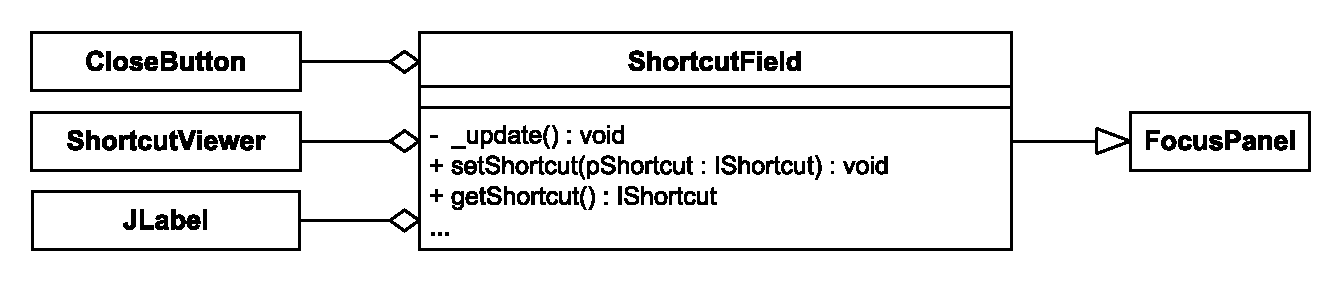
\includegraphics[width=0.8\linewidth]{../graphic/diagrams/CD_ShortcutField/ShortcutField}
	\caption{ShortcutField}
	\label{fig:shortcutfield}
\end{figure}

Die eigentliche Funktionalität wird durch die verwendeten Komponenten bereitgestellt. Das \emph{ShortcutField} kümmert sich selber lediglich um die Anzeige der jeweils richtigen Komponente (\emph{JLabel} oder \emph{ShortcutView}), sowie um das Horchen auf Tastatureingaben mittels eines \emph{KeyListeners}. Die private Methode \emph{\_update()} ist für das Ein- und Ausblenden der jeweiligen Komponente zuständig (siehe \autoref{fig:ShortcutField-update}). Sie wird initial und bei jeder Änderung des Shortcuts aufgerufen.

\vspace{20px}

\begin{wrapfigure}[11]{l}[0cm]{0.50\textwidth}
    \centering
	\vspace{-5px}
	\begin{spacing}{0.75}
		\begin{javacode}[firstnumber=205]
private void _update()
{
  boolean empty = getShortcut() == null;
	
  viewerContainer.setVisible(!empty);
  textContainer.setVisible(empty);
  
  crossButton.setVisible(isEditable());
  crossButton.setEnabled(!empty);
}		\end{javacode}
	\end{spacing}
	\caption{Ein- und Ausblenden der Komponenten}
	\label{fig:ShortcutField-update}
\end{wrapfigure}

Zunächst wird überprüft, ob das \emph{ShortcutField} leer ist (kein Shortcut gesetzt). Das Ergebnis dieser Überprüfung wird in der lokalen Variable \emph{empty} gespeichert. Anschließend werden die Sichtbarkeiten der Komponenten aktualisiert, wobei der \emph{ShortcutViewer} nur bei gesetztem und die Textaufforderung nur bei nicht gesetztem Tastenkürzel angezeigt wird. Der \emph{CrossButton} wird im Editiermodus immer angezeigt aber nur aktiviert, sobald ein Shortcut eingegeben wird.

\newpage

\subsubsection{Check-Button}

\vspace{-3px}

Um die Grundfunktionalität des im Abschnitt \ref{ui} erwähnten Check-Buttons zu definieren, wurde zunächst das Interface \emph{ICheckComponent} erstellt. Indessen wird festgelegt, dass ein Check-Button einen Checked-Zustand besitzt, welcher angibt, ob innerhalb der Komponente ein grüner Haken (\emph{true}) oder ein rotes Kreuz (\emph{false}) angezeigt werden soll (siehe \autoref{fig:cdcheckbutton}).

Die Klasse \emph{CheckToggleButton} implementiert das beschriebene Interface und erbt von der Swing Klasse \emph{JToggleButton}. Sie kümmert sich um das Einfügen und Aktualisieren des richtigen Symbols. Innerhalb von \emph{setChecked(...)} wird die private Methode \emph{\_updateIcon()} aufgerufen, welche ihrerseits das jeweilige Symbol über das gesetzte Icon zeichnet (siehe Anhang \ref{CheckToggleButton}). Insgesamt stellt ein \emph{CheckToggleButton} eine vollwertige CheckComponent dar, welche direkt verwendet werden könnte.

\begin{figure}[H]
	\centering
	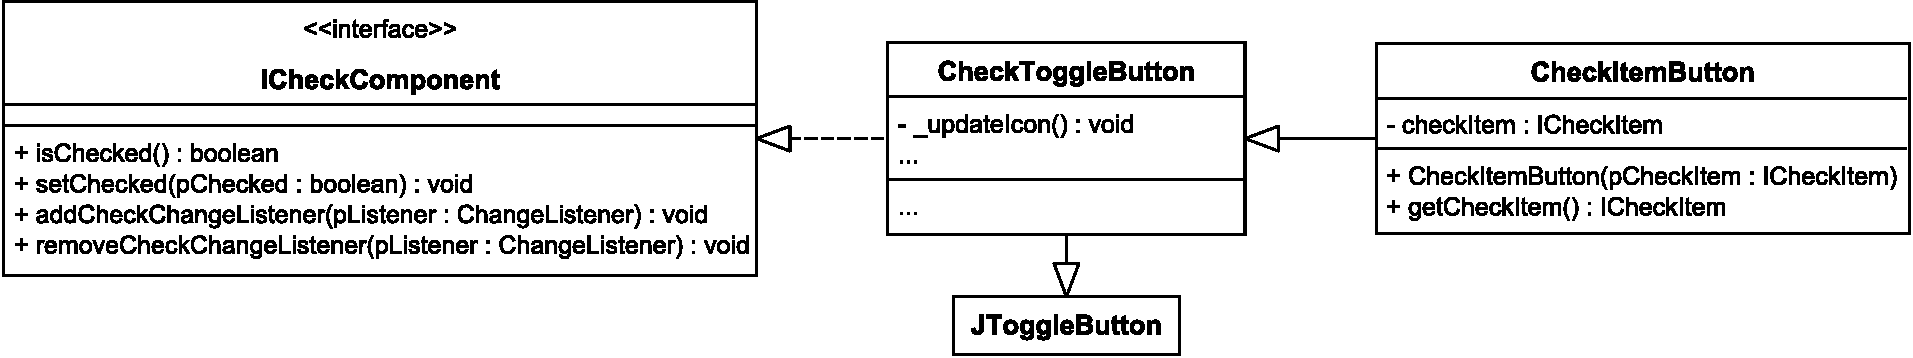
\includegraphics[width=1\linewidth]{../graphic/diagrams/CD_CheckButton/CD_CheckButton}
	\caption{CheckItemButton}
	\label{fig:cdcheckbutton}
\end{figure}

\vspace{-9px}

Um die Benutzung von \emph{CheckToggleButtons} innerhalb des Shortcut Editors bzw. im Zusammenhang mit \emph{ICheckItems} einfacher zu gestalten, wurde die Klasse \emph{CheckItemButton} eingeführt. Diese erweitert \emph{CheckToggleButton} und kann über den Konstruktor ein \emph{ICheckItem} aufnehmen. Wie im Anhang \ref{CheckItemButton} ersichtlich, werden innerhalb dieses Konstruktors alle Eigenschaften entsprechend dem \emph{ICheckItem} gesetzt (z. B. Checked-Zustand oder Icon).

\vspace{-9px}

\subsubsection{CheckItemContainer}

\vspace{-3px}

\begin{wrapfigure}[15]{r}[0cm]{165px}
	\vspace{-12px}
	\centering
	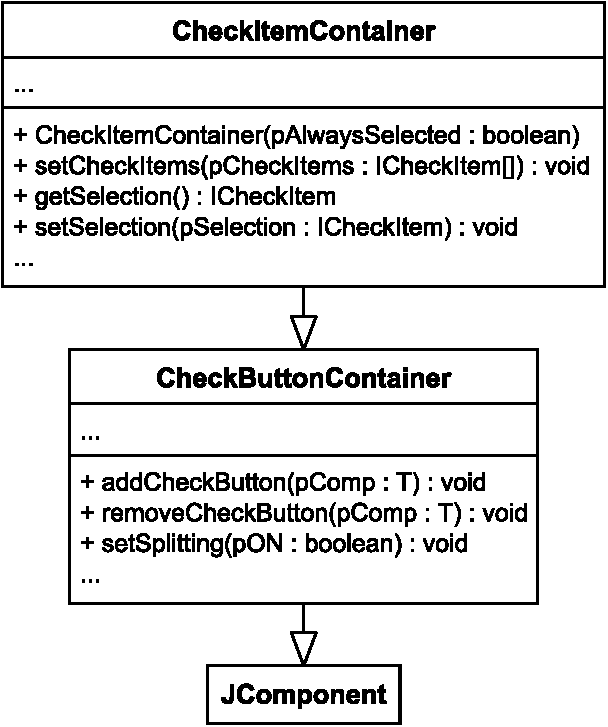
\includegraphics[width=.95\linewidth]{../graphic/diagrams/CD_CheckItemContainer/CD_CheckItemContainer}
	\caption{CheckItemContainer}
	\label{fig:cdcheckitemcontainer}
\end{wrapfigure}

Der Designentwurf lässt erkennen, dass die Check-Buttons einer bestimmten Positionierung bzw. Sortierung unterliegen: Auf der linken Seite befinden sich alle unchecked und auf der rechten Seite alle checked Buttons. Zudem wird bei den Check-Buttons zur Auswahl des Browsers ein Abstand zwischen den beiden Buttongruppen eingefügt. 

Um diese Positionierung zu realisieren, wurde der \emph{CheckItemContainer} erstellt. Dieser stellt eine \emph{JComponent} dar, welcher mittels eines \emph{BoxLayouts} seine CheckButtons horizontal nebeneinander ausrichtet. Um den zuvor erwähnten Abstand ein- und auszuschalten, existiert die Methode \emph{setSplitting(...)}, welche einen \emph{boolean} erwartet. Ändert sich der Checked-Zustand eines CheckButtons, so kümmert sich der Container auch um die richtige Umsortierung.

Um wiederum die Nutzung innerhalb des Shortcut Editors zu erleichtern, existiert der \emph{CheckItemContainer}. Diesem kann man \emph{CheckItems} setzten (\emph{setCheckItems(...)}), wonach dieser intern die benötigten Check-Buttons erzeugt und sich selbst hinzufügt oder Unnötige wieder entfernt (siehe Anhang \ref{CheckItemContainer}). Zudem kann über die Methode \emph{getSelection()} der aktuell selektierte Check-Button ausgelesen werden.

\subsubsection{CheckItemAccordion}

\vspace{-8px}

Die Accordion-Komponente ist in der Lage, einen konkreten Pfad des Datenmodells für Browsertestergebnisse mit allen verfügbaren Details darzustellen (siehe \autoref{fig:uxDesigns}).
Jede Sektion des Accordions visualisiert genau ein CheckItem. Sofern Untersektionen vorhanden sind, wird zusätzlich ein CheckItemContainer angezeigt. Dieser dient zur Navigation durch das Datenmodell, wobei immer genau das CheckItem dargestellt wird, welches in der vorherigen Sektion ausgewählt ist.

\begin{wrapfigure}[10]{l}[0cm]{230px}
	\vspace{-12px}
	\centering
	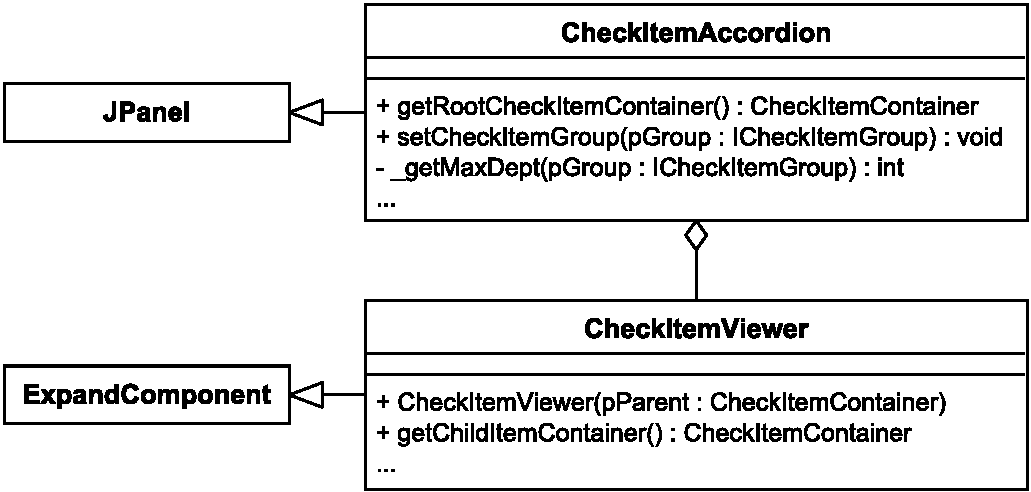
\includegraphics[width=0.95\linewidth]{../graphic/diagrams/CD_CheckItemAccordion/CheckItemAccordion}
	\caption{CheckItemAccordion}
	\label{fig:checkitemaccordion}
\end{wrapfigure}


Das \emph{CheckItemAccordion} erbt von der Swing Klasse \emph{JPanel} (siehe \autoref{fig:checkitemaccordion}) und verwendet zur vertikalen Positionierung der einzelnen Sektionen das \emph{BoxLayout}. Im Konstruktor wird der oberste \emph{CheckItemContainer} erzeugt, welcher zur Auswahl des Browsers dient und sich nicht innerhalb des Accordions befindet (siehe \autoref{fig:uxDesigns}). Um auf diesen außerhalb zugreifen zu können, dient die Methode \emph{getRootCheckItemContainer()}.

Eine Sektion wird durch die Klasse \emph{CheckItemViewer} repräsentiert (siehe \autoref{fig:checkitemaccordion}). Diese Komponente besitzt die Fähigkeit, alle Details eines CheckItems in tabellarischer Form darzustellen. Sie erbt von \emph{ExpandComponent}, wodurch die Funktion des Ein- und Ausklappens und die Anzeige einer Header-Leiste ermöglicht wird. Damit das selektierte \emph{CheckItem} des vorherigen \emph{CheckItemViewers} angezeigt und auf Selektionsänderungen reagiert werden kann, wird im Konstruktor der vorherige \emph{CheckItemContainer} übergeben. Diesem wird ein Listener hinzugefügt, welcher auf Änderungen der Selektion horcht und so die Aktualisierung des Viewers ermöglicht.

\begin{wrapfigure}[16]{r}[0px]{322px}
    \centering
	\vspace{-5px}
	\begin{spacing}{0.75}
		\begin{javacode}[firstnumber=62]
public void setCheckItemGroup(ICheckItemGroup pRootGroup)
{
  if(!Objects.equals(pRootGroup, rootGroup))
  {
    rootGroup = pRootGroup;
    
    rootCheckItemContainer.setCheckItems(pRootGroup.getItems());
    
    int dept = _getMaxDept(pRootGroup);
    CheckItemContainer children = rootCheckItemContainer;
    
    removeAll();
    for (int i = 0; i < dept; i++)
    {
      CheckItemViewer viewer = new CheckItemViewer(children);
      children = viewer.getChildItemContainer();
      add(viewer);
    }
  }
}\end{javacode}
	\end{spacing}
	\caption{Setzten der CheckItemGroup im CheckItemAccordion}
	\label{fig:CheckItemAccordion-setCheckItemGroup}
\end{wrapfigure}

In \autoref{fig:CheckItemAccordion-setCheckItemGroup} ist der Sourcecode der Methode \emph{setCheckItemGroup(...)} abgebildet. In dieser wird anhand der übergebenen \emph{ICheckItemGroup} das Accordion aufgebaut. Zu Beginn wird überprüft, ob es sich bei der übergebenen Gruppe um die bereits gesetzte handelt. Ist dies der Fall, so wird die Methode ohne Änderungen verlassen. Andernfalls werden dem RootCheckItemContainer die CheckItems der RootGruppe (Browser Check-Items) gesetzt. Anschließend wird über die Methode \emph{\_getMaxDept(...)} die maximale Tiefe der Baumstruktur von \emph{pRootGroup} ermittelt. Dieses Ergebnis dient als Grundlage für die Anzahl von Sektionen, die eingefügt werden. Nach dem Löschen aller vorhandenen Komponenten wird in jedem Schleifendurchgang eine Sektion eingefügt. Dabei wird im Konstruktor des \emph{CheckItemViewers} immer der \emph{CheckItemContainer} der vorherigen Sektion oder am Anfang der \emph{rootCheckItemContainer} übergeben. Dadurch wird der richtige Zusammenhang zwischen den Sektionen hergestellt.

\subsubsection{BreadCrumb und TreeTable}

Die Komponenten BreadCrumb und TreeTable mussten im Zuge dieser Projektarbeit nicht neu entwickelt werden, da sie bereits zu einem früheren Zeitpunkt umgesetzt wurden. 

\begin{wrapfigure}[12]{l}[0cm]{230px}
	\vspace{-12px}
	\centering
	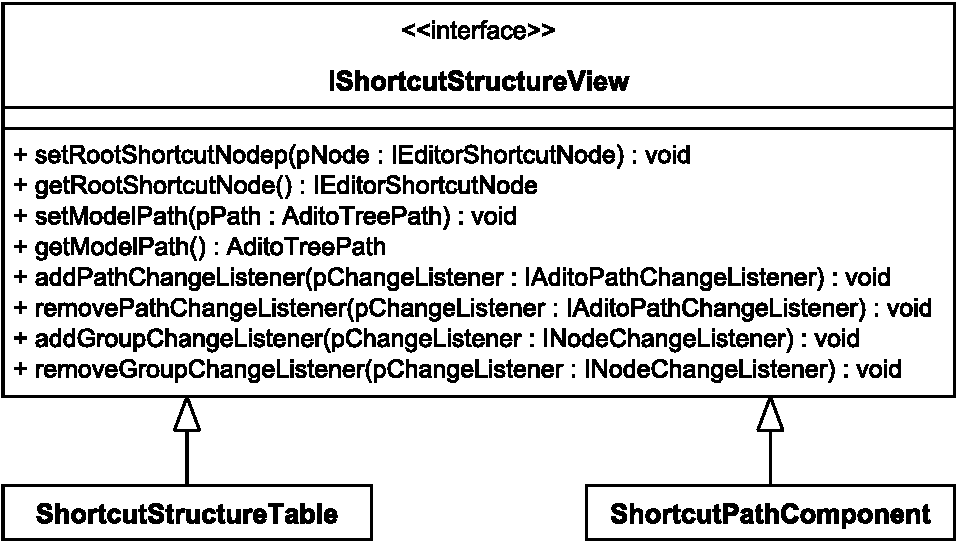
\includegraphics[width=1\linewidth]{../graphic/diagrams/CD_IShortcutStructureView/IShortcutStructureView}
	\caption{IShortcutStructureView}
	\label{fig:ishortcutstructureview}
\end{wrapfigure}

Um sie jedoch im Zusammenhang mit dem MVP-Architekturmuster verwenden zu können, mussten sie in eigene Klassen gekapselt werden, welche \emph{IShortcutStructureView} (siehe \autoref{fig:ishortcutstructureview}) implementieren. Dazu wurden die Klassen \emph{ShortcutPathComponent} (BreadCrumb) und \emph{ShortcutStructureTable} (TreeTable) erstellt (siehe Anhang \ref{ShortcutStructureTable} und \ref{ShortcutPathComponent}). Über die im Interface enthaltenen Methoden erhält die jeweilige Komponente ihre Informationen, welche zur Darstellung benötigt werden. Außerdem erhält sie die Möglichkeit, Wertänderungen über Listener zu kommunizieren. Wählt der Benutzer beispielsweise einen anderen Knoten in der BreadCrumb aus, so werden alle hinzugefügten \emph{PathChangeListener} informiert.


\subsubsection{ShortcutEditorUI}

Nach Implementierung der einzelnen Komponenten mussten diese zu einem gesamten User Interface zusammengesetzt werden. Hierzu wurde die Klasse \emph{ShortcutEditorUI} (siehe Anhang \ref{ShortcutEditorUI}) erstellt. Sie implementiert das Interface \emph{IShortcutEditorUI}, welches wiederum von \emph{IShortcutStructureView} erbt. Zudem erbt die UI von der Swing Klasse \emph{JPanel} (\autoref{fig:shortcuteditorui}).

\begin{figure}[H]
	\centering
	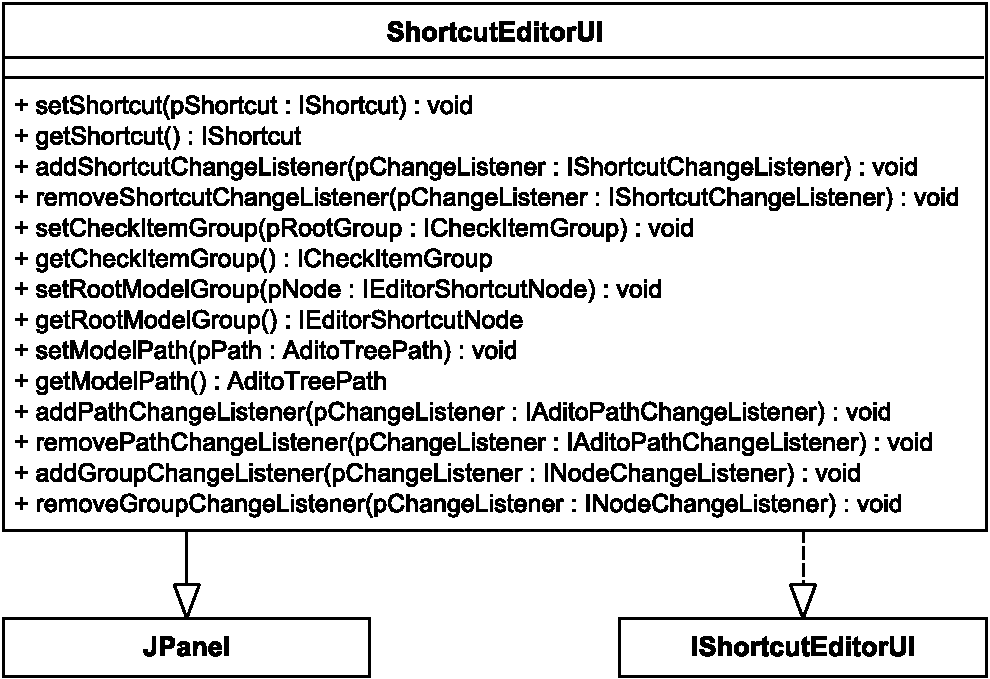
\includegraphics[width=1\linewidth]{../graphic/diagrams/CD_ShortcutEditorUI/ShortcutEditorUI}
	\caption{ShortcutEditorUI}
	\label{fig:shortcuteditorui}
\end{figure} 

\vspace{-12px}

Zur Anordnung der einzelnen Komponenten kommt das \emph{TableLayout} zum Einsatz. Im Konstruktor der Klasse werden die Spalten- und Zeilenausdehnungen des Layouts definiert und die Komponenten in die entsprechenden Zellen eingefügt. Außerdem werden das \emph{ShortcutStructureModel} und der \emph{ShortcutStructurePresenter} initialisiert. 

Da die Funktionalität in den für die UI verwendeten Komponenten enthalten ist, werden alle Getter- und Setter-Anfragen sowie die Listener direkt an das entsprechende Element (Komponente oder Model) weitergeleitet. In der \emph{setShortcut(...)} Methode der ShortcutEditorUI wird beispielsweise sofort die \emph{setShortcut(...)} Methode des ShortcutFields aufgerufen und so der zu setzende Shortcut direkt weitergegeben.

\newpage

\subsection{Presenter}

Folgend wird die Implementierung der im Abschnitt \ref{Architekturdesign} beschriebenen Presenter erläutert.

\subsubsection{ShortcutEditorPresenter}

\begin{wrapfigure}[11]{r}[0cm]{230px}
	\vspace{-12px}
	\centering
	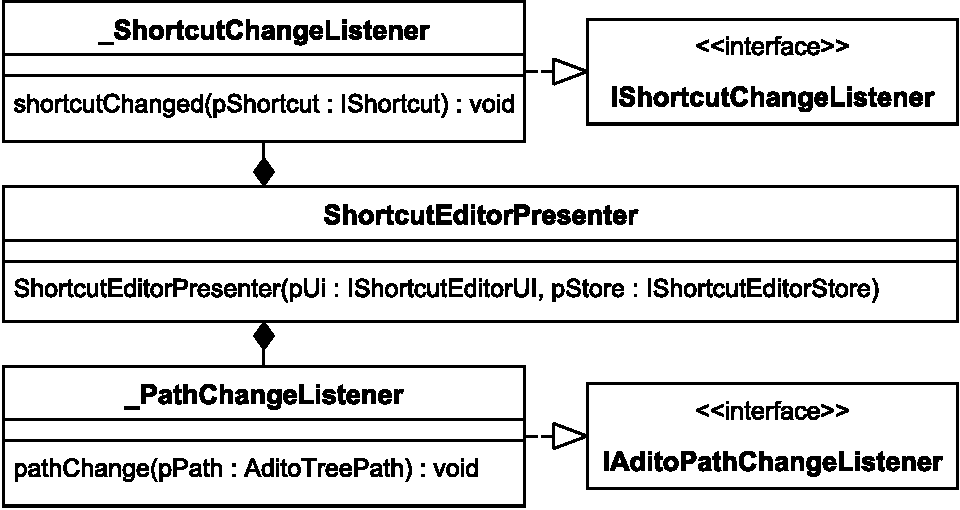
\includegraphics[width=230px]{../graphic/diagrams/CD_ShortcutEditorPresenter/ShortcutEditorPresenter}
	\caption{ShortcutEditorPresenter}
	\label{fig:shortcuteditorpresenter}
\end{wrapfigure}

Um die Daten der \emph{ShortcutEditorUI} mit den in Abschnitten \ref{DatenmodellFunc} und \ref{DatenmodellBrow} beschriebenen Datenmodellen abzugleichen, existiert gemäß des MVP-Architekturmusters der \emph{ShortcutEditorPresenter} (siehe Anhang \ref{ShortcutEditorPresenter}). Diesem wird über den Konstruktor sowohl der DataStore als auch eine \emph{IShortcutEditorUI} übergeben. Anschließend werden die UI Listener hinzugefügt, welche auf Shortcut- und Pfadänderungen horchen.

Ändert der Benutzer über die UI den Shortcut, so wird dieser in das entsprechende Datenmodell übertragen. Wird durch den Benutzer der Pfad geändert, also eine andere Aktion selektiert, so lädt der Presenter das Datenmodell der neuen Aktion. Zukünftige Shortcutänderungen werden dann in dieses Datenmodell übertragen.

\subsubsection{ShortcutStructurePresenter}

Da bei den beiden Komponenten TreeTable und BreadCrumb dieselben Daten präsentiert werden, kommt zur Abgleichung ebenfalls das MVP-Architekturmuster zum Einsatz, wobei die beiden genannten Komponenten die Views darstellen. Der Presenter (siehe Anhang \ref{ShortcutStructurePresenter}) erhält über den Konstruktor ein \emph{ShortcutStructureModel} und eine beliebige Anzahl von \emph{IShortcutStructureViews}. 

In \autoref{fig:ishortcutstructureview} wird ersichtlich, dass eine View einen \emph{IEditorShortcutNode} und einen \emph{AditoTreePath} besitzt. Der \emph{IEditorShortcutNode} hält die in Abschnitt \ref{DatenmodellFunc} beschriebene Baumstruktur der Aktionen und der Pfad gibt an, welcher Knoten des Baums selektiert ist. Über Änderung dieser Attribute informieren Listener, welche der View über die entsprechenden Methoden hinzugefügt werden können (z. B. \emph{addPathChangeListener(...)}). Da das \emph{ShortcutStructureModel} die gleiche Funktionalität benötigt, wie die View, implementiert es auch das Interface \emph{IShortcutStructureView} (siehe Anhang \ref{ShortcutStructureModel}).

Im Konstruktor des \emph{ShortcutStructurePresenters} (siehe Anhang \ref{ShortcutStructurePresenter}) werden sowohl dem Model als auch den einzelnen Views Pfad- und Node-Listener hinzugefügt. Löst ein Listener des Models aus, so werden die Änderungen in alle Views übertragen. Löst ein Listener einer View aus, so werden die Änderungen in das Model übertragen. Da dadurch wiederum der Listener des Models anschlägt, werden auch die anderen Views aktualisiert. So wird gewährleistet, dass alle Views und das Model zu jedem Zeitpunkt die gleichen Informationen besitzen.

\begin{figure}[H]
	\centering
	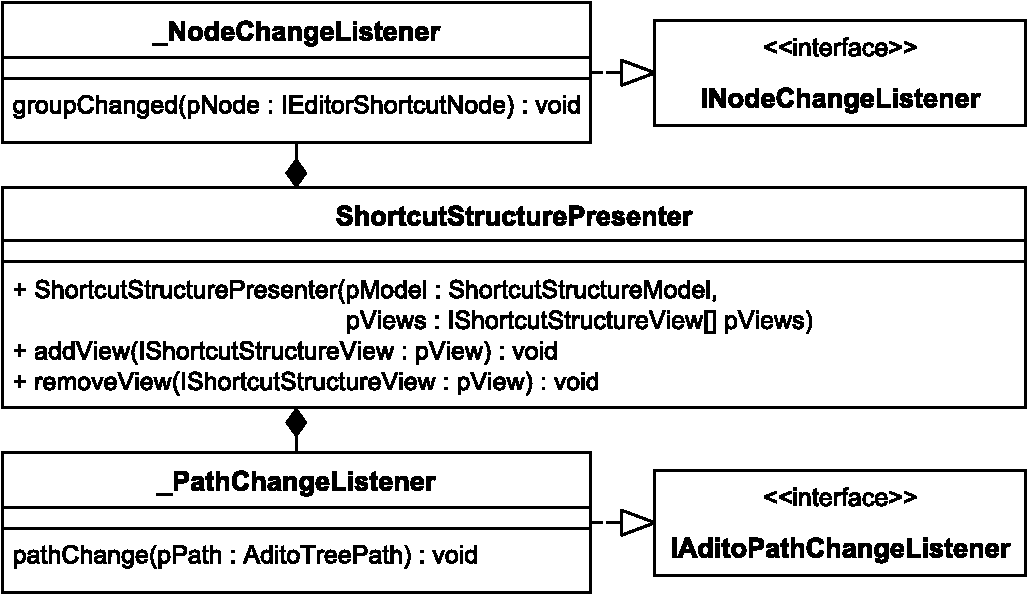
\includegraphics[width=0.6\linewidth]{../graphic/diagrams/CD_ShortcutStructurePresenter/ShortcutStructurePresenter}
	\caption{ShortcutStructurePresenter}
	\label{fig:shortcutstructurepresenter}
\end{figure}

\newpage
\section{Anwendungstests}

\section{Fazit}
\par Der produktive Einsatz des Remote-Loggers wird weitere Anforderungen der Administratoren und ADITO4-Projektentwickler aufzeigen. Es wurde hierdurch eine Möglichkeit geschaffen, direkt auf die Ausgaben des ADITO4-Servers zuzugreifen. Das hat den Vorteil, dass nun nicht mehr per Fernzugriff auf das Hostsystem der ADITO4-Kundenserver verbunden werden muss, um dessen Meldungen zu lesen. \\
Der Remote-Logger bietet auch im Vergleich zum bisherigen \glqq FileLogger\grqq\ den entscheidenden Echtzeit-Vorteil, denn der ADITO4-FileLogger schreibt alle erhaltenen CheckPoints blockweise in seine Datei. Somit werden Ausgaben verzögert geschrieben und es kann erst verspätet auf diese reagiert werden.

\par Es ist denkbar, dass das Feature des Remote-Loggers noch mit einer Exportfunktion erweitert wird. Somit könnte man Log-Dateien erstellen, die man wiederum mit dem \glqq LogFileViewer\grqq\ des ADITO4-Managers betrachten kann. \\
Ebenso wäre es möglich einen Filter zu implementieren, der alle Nachrichten die der Benutzer nicht sehen möchte, herausfiltert. Beispielweise werden dann nur noch Nachrichten mit der Priorität \glqq hoch\grqq\ angezeigt. Einstellbar soll dies mit verschiedenen Buttons und Eingabefelder werden. Ein Filter nach angemeldeten Benutzern ist von der ADITO-Geschäftsleitung ebenfalls gewünscht, denn somit könnten auftretende Fehler am ADITO4-Client leichter identifiziert und behoben werden. \\
Eine zusätzliche Erweiterung des Remote-Loggers könnte die Verschlüsselung des Datenaustausches zwischen Remote-Logger-Server und Remote-Logger-Client sein. Dann könnte nahezu komplett ausgeschlossen werden, dass unberechtigte Dritte Zugriff zu den vom Remote-Logger-Server gesendeten Daten erhalten. Hierzu käme SSL in Frage. SSL wurde bereits bei der Kommunikation zwischen ADITO4-Server und ADITO4-Client verwendet, was ein Wiederverwenden von bereits bestehendem Code erlaubt.
\newpage

\section{Glossar}
\begin{center}
	\begin{tabularx}{\textwidth}{p{.3\textwidth}|X}
	    CheckPoint  & Ein CheckPoint kapselt entweder eine Informationsmeldung oder eine Fehlermeldung der ADITO-Softwareprodukte. Diese besteht aus einer Nachricht und mehreren IDs für Programm, Priorität und Art/Ursache (siehe \prettyref{sec:IRemoteLoggerCommand}) \\

   	  	Consumer  & Das Java-spezifische Interface \glqq Consumer\grqq\ repräsentiert eine Operation, die ein einzelnes Argument annimmt und kein Ergebnis zurückgibt \\

	    CRM / xRM & 
		Customer Relationship Management / Any Relationship Management
	  	Steht für Kundenpflege/-bindung, Datensammlung, Datenpflege, Datenverwaltung und das Ziel, Kundenpotenziale optimal auszuschöpfen \\ 
	  	
	  	Fassade (Facade) & Eine Fassade bietet eine einheitliche Schnittstelle zu einer Menge von Schnittstellen eines Subsystems. Vereinfacht die Benutzung des Subsystems.\\
	  	
	  	Java-Network-API & Leicht benutzbare Netzwerk-API der Programmiersprache Java. Diese erlaubt es auf bestimmte Netzwerkadressen des Computers zu hören und Nachrichten über das Netzwerk zu senden \\
	  	
	  	Logging & Unter Logging versteht man das Speichern von Prozessen oder Datenänderungen. Diese werden in sogenannten Logdateien hinterlegt bzw. gespeichert. Dies wird in Java meist mit Hilfe der modularen Log4J-API abgebildet.\\
	  	
	  	Logdatei  & Eine Logdatei enthält das automatisch geführte Protokoll bestimmter Aktionen von Prozessen auf einem Computersystem. \\
	  	
	  	Remote & Remote bedeutet entfernt, wobei die Entfernung sich darauf bezieht, dass der Benutzer keinen unmittelbaren Kontakt mit dem Remote-Gerät hat.\\
	  	
	  	serialisierbares Objekt  & Bezeichnet ein Objekt, das in einen Datenstrom umgewandelt werden und somit über das Netzwerk gesendet werden kann. \\

	\end{tabularx}
\end{center}
\newpage

\section{Abbildungsverzeichnis}
\vspace{-25px}
\renewcommand*\listfigurename{}
\listoffigures
\thispagestyle{fancy}
\section{Literaturverzeichnis}
\begin{itemize}
\item Riehle, Dirk (1996): \glqq Entwurfsmuster\grqq
\end{itemize}
\newpage

\section{Anhang}
\addtocontents{toc}{\protect\setcounter{tocdepth}{-1}}

\subsection{Anwendungsfälle}

\vfill
\begin{figure}[H]
	\centering
	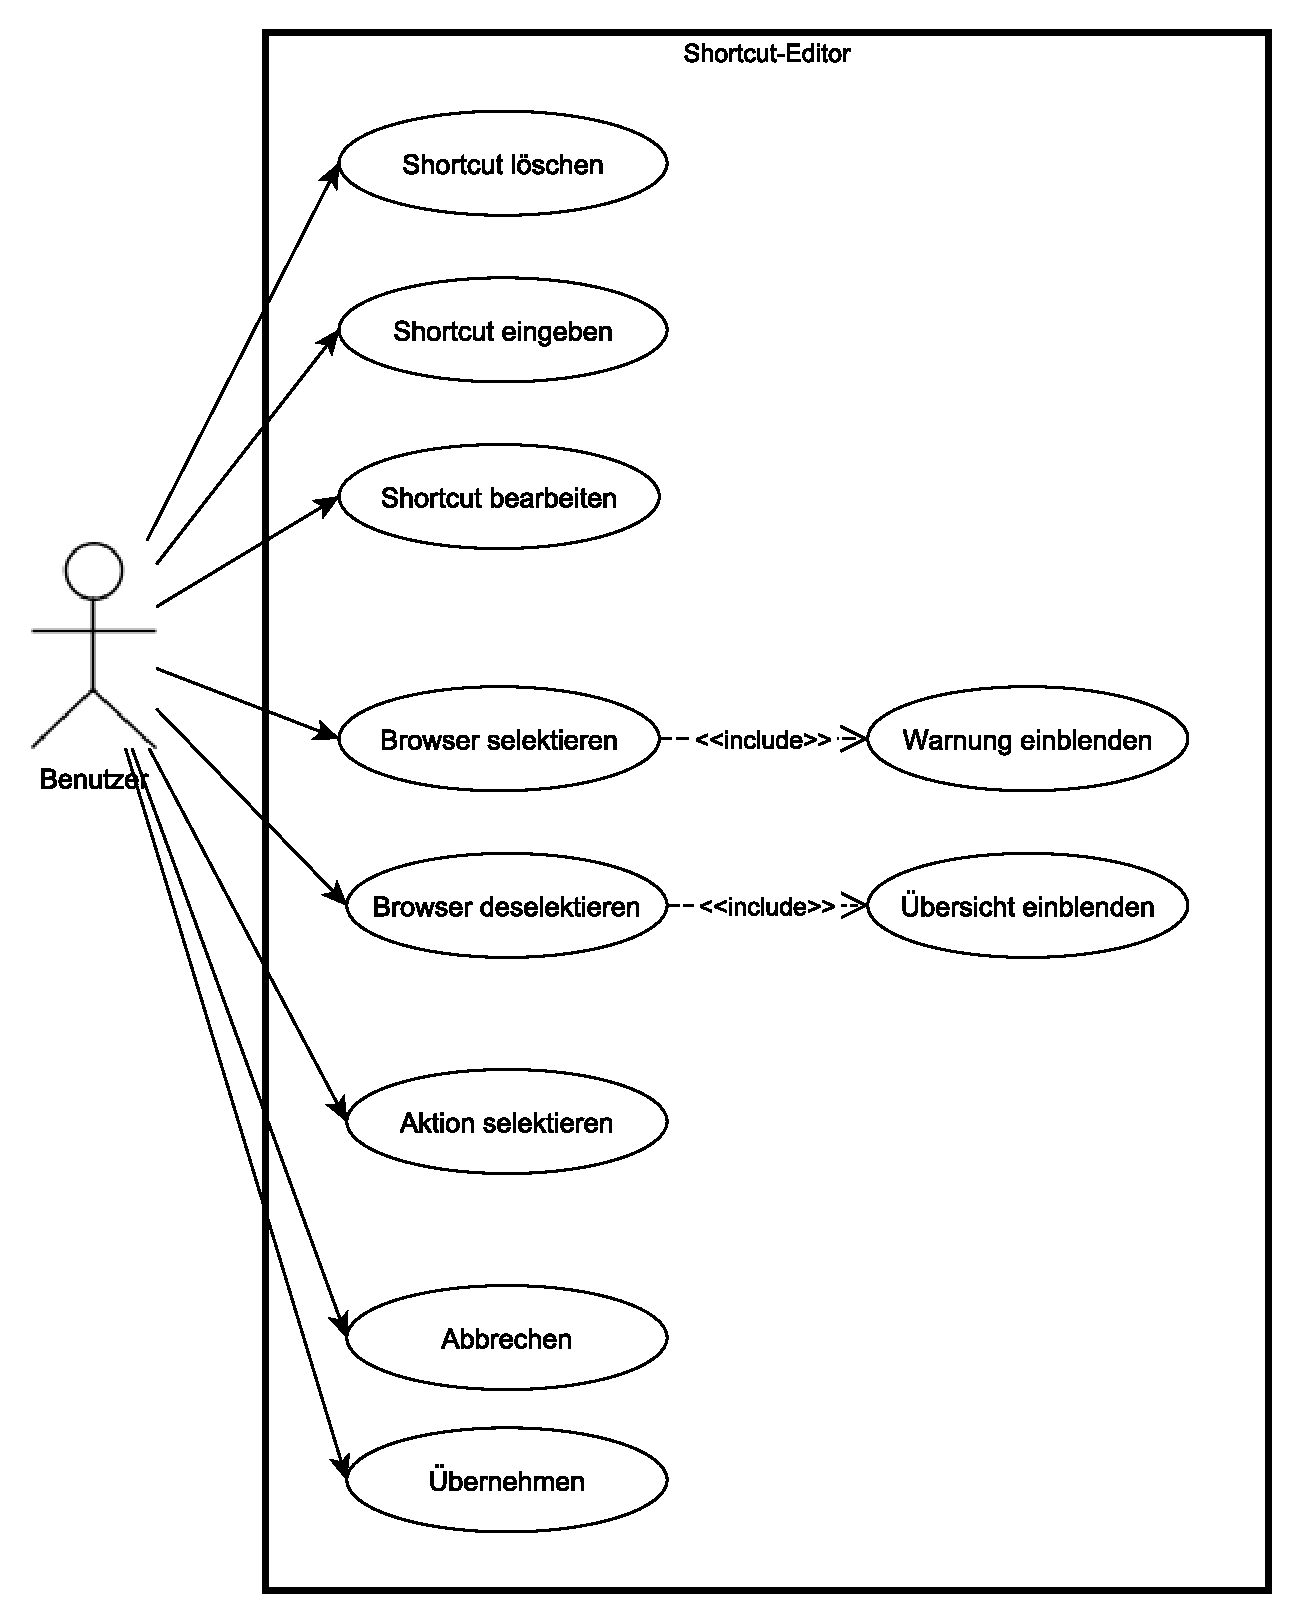
\includegraphics[width=\linewidth]{../graphic/diagrams/UC_Anwendungsfall/Anwendungsfall}
	\caption{Use-Case-Diagramm}
	\label{fig:anwendungsfall}
\end{figure}
\vfill

\newpage

\subsection{Verwendete Ressourcen}
\label{ressources}

\textbf{Hardware}

\begin{itemize}
\item Büroarbeitsplatz (PC, Tastatur, Maus etc.)
\end{itemize}
 
\textbf{Software}

\begin{itemize}
\item Windows 10 Professional – Betriebssystem
\item IntelliJ IDEA – Entwicklungsumgebung Java
\item Java JDK - Software Developer Kit (SDK)
\item Maven - Buildsystem
\item git – Verteilte Versionsverwaltung
\item MiKTeX – Distribution des Textsatzsystems \LaTeX
\item TeXstudio – Entwicklungsumgebung für \TeX
\item yEd Graph Editor - Anwendung zur Erstellung von UML-Diagramme
\end{itemize}

\textbf{Personal}

\begin{itemize}
\item Mitarbeiter der UX-Abteilung – Erstellung von Designentwürfen
\item Entwickler – Umsetzung des Projektes
\end{itemize}


\end{document}